%%%%%%%%%%%%%%%%%%%%%%% file template.tex %%%%%%%%%%%%%%%%%%%%%%%%%
%
% This is a general template file for the LaTeX package SVJour3
% for Springer journals.          Springer Heidelberg 2010/09/16
%
% Copy it to a new file with a new name and use it as the basis
% for your article. Delete % signs as needed.
%
% This template includes a few options for different layouts and
% content for various journals. Please consult a previous issue of
% your journal as needed.
%
%%%%%%%%%%%%%%%%%%%%%%%%%%%%%%%%%%%%%%%%%%%%%%%%%%%%%%%%%%%%%%%%%%%
%
% First comes to an example EPS file -- just ignore it and
% proceed on the \documentclass line
% your LaTeX will extract the file if required
%
\RequirePackage{fix-cm}
%
%\documentclass{svjour3}                     % onecolumn (standard format)
%\documentclass[smallcondensed]{svjour3}     % onecolumn (ditto)
\documentclass[smallextended]{svjour3}       % onecolumn (second format)
%\documentclass[twocolumn]{svjour3}          % twocolumn
%
\smartqed  % flush right qed marks, e.g. at the end of proof
%
\usepackage{graphicx}
\usepackage{tabularx}
\usepackage{amsmath,mathptmx,amssymb}
\usepackage{bm}
% \usepackage[utf8]{inputenc}
\usepackage{color}
\usepackage{subfig}
\usepackage{todonotes}

\sloppy\hyphenpenalty 1000000

%
% \usepackage{mathptmx}      % use Times fonts if available on your TeX system
%
% insert here the call for the packages your document requires
%\usepackage{latexsym}

\usepackage{algorithmicx} 
% \usepackage{algorithmic}
\usepackage{algorithm}
\usepackage{algpseudocode}
\usepackage{array}
\newcolumntype{P}[1]{>{\centering\arraybackslash}p{#1}}
\newcolumntype{M}[1]{>{\centering\arraybackslash}m{#1}}
\usepackage{hyperref}
\hypersetup{
    colorlinks=true,
    linkcolor=blue,
    filecolor=blue,
    citecolor=blue,
    urlcolor=blue,
    }
\renewcommand\UrlFont{\color{blue}\rmfamily}
\usepackage{xcolor}
\usepackage{graphicx} %Loading the package
\graphicspath{{./img/}} %Setting the graphicspath
%
% please place your own definitions here and do not use \def but
% \newcommand{}{}
%
% Insert the name of "your journal" with
% \journalname{myjournal}
%
\begin{document}

\title{
An evolutionary approach with feature engineering  for drought prediction
}
% \subtitle{Do you have a subtitle?\\ If so, write it here}

%\titlerunning{Short form of title}        % if too long for running head

\author{
%         Igor Michel Santos Leite \and
%         Jo\~ao Daniel Madureira Yamim\and
        Leonardo Goliatt  {\large *}
        }

%\authorrunning{Short form of author list} % if too long for running head

\institute{
%            Igor Michel Santos Leite (corresponding author) \at
%               Computational modelling, Federal University of Juiz de Fora, Brazil \\
%               \email{igor.leite@ice.ufjf.br}           %  \\
%            \and
%           João Daniel Madureira Yamim \at
%               Computational modelling, Federal University of Juiz de Fora, Brazil \\
%               \email{joao.yamim@engenharia.ufjf.br}           %  \\
%            \and
          {\large *} L. Goliatt  \at
              Computational Modelling Program, Federal University of Juiz de Fora, Brazil \\
              \email{leonardo.goliatt@ufjf.edu.br}         %  \\
}

\date{Received: date / Accepted: date}


\maketitle              % typeset the header of the contribution
%
\begin{abstract}

\keywords{Drought prediction \and differential evolution \and calibration \and Heston model \and Monte Carlo simulation}
\end{abstract}
%
%
%
\section{Introduction}\label{sec:intro}


Mehr et and collaborators \cite{danandehmehr2020neuroannealing}
presented a new hybrid model, called ENN-SA, for spatiotemporal drought prediction. In ENN-SA, an Elman neural network (ENN) is conjugated with simulated annealing (SA) optimization and support vector machine (SVM) classification algorithms for the standardized precipitation index (SPI) modeling at multiple stations.



Mehr et al \cite{danandehmehr2020neurofuzzy} presented a tree-based model, namely
Fuzzy Random Forest (FRF), for one month ahead Standardized
Precipitation Evapotranspiration Index (SPEI) classification and
prediction with a noteworthy application in ungauged catchments.


\section{Material and Methods}\label{sec:prob_formulation}

\subsection{Study area and dataset}

\subsection{Feature engineering}

\subsection{Lasso linear model}

The Lasso \cite{tibshirani1996lasso} minimizes the residual sum of squares subject to the sum of the absolute value of the coefficients being less than a constant. Because of the nature of this constraint it tends to produce some coefficients that are exactly 0 and hence gives interpretable models. 
% Our simulation studies suggest that the lasso enjoys some of the favourable properties of both subset selection and ridge regression. It produces interpretable models like subset selection and exhibits the stability of ridge regression. There is also an interesting relationship with recent work in adaptive function estimation by Donoho and Johnstone. The lasso idea is quite general and can be applied in a variety of statistical models: extensions to generalized regression models and tree-based models are briefly described.

\subsection{Time-series cross-validation}

The use of machine learning models in data from time series requires special care due to their peculiarities. One must choose the test set within a period of time after the training set. Otherwise, some information may leak from the training set to the training set, compromising the learning process of the machine learning model. A more robust solution is to operate similarly to k-fold cross-validation but in a time-ordered way. The figure below illustrates the cross-validation procedure for time series. By training and adjusting the model in training set for each fold and averaging the errors in the test sets, we can obtain an unbiased estimate of the model's performance.

\begin{figure}[!htb]\centering
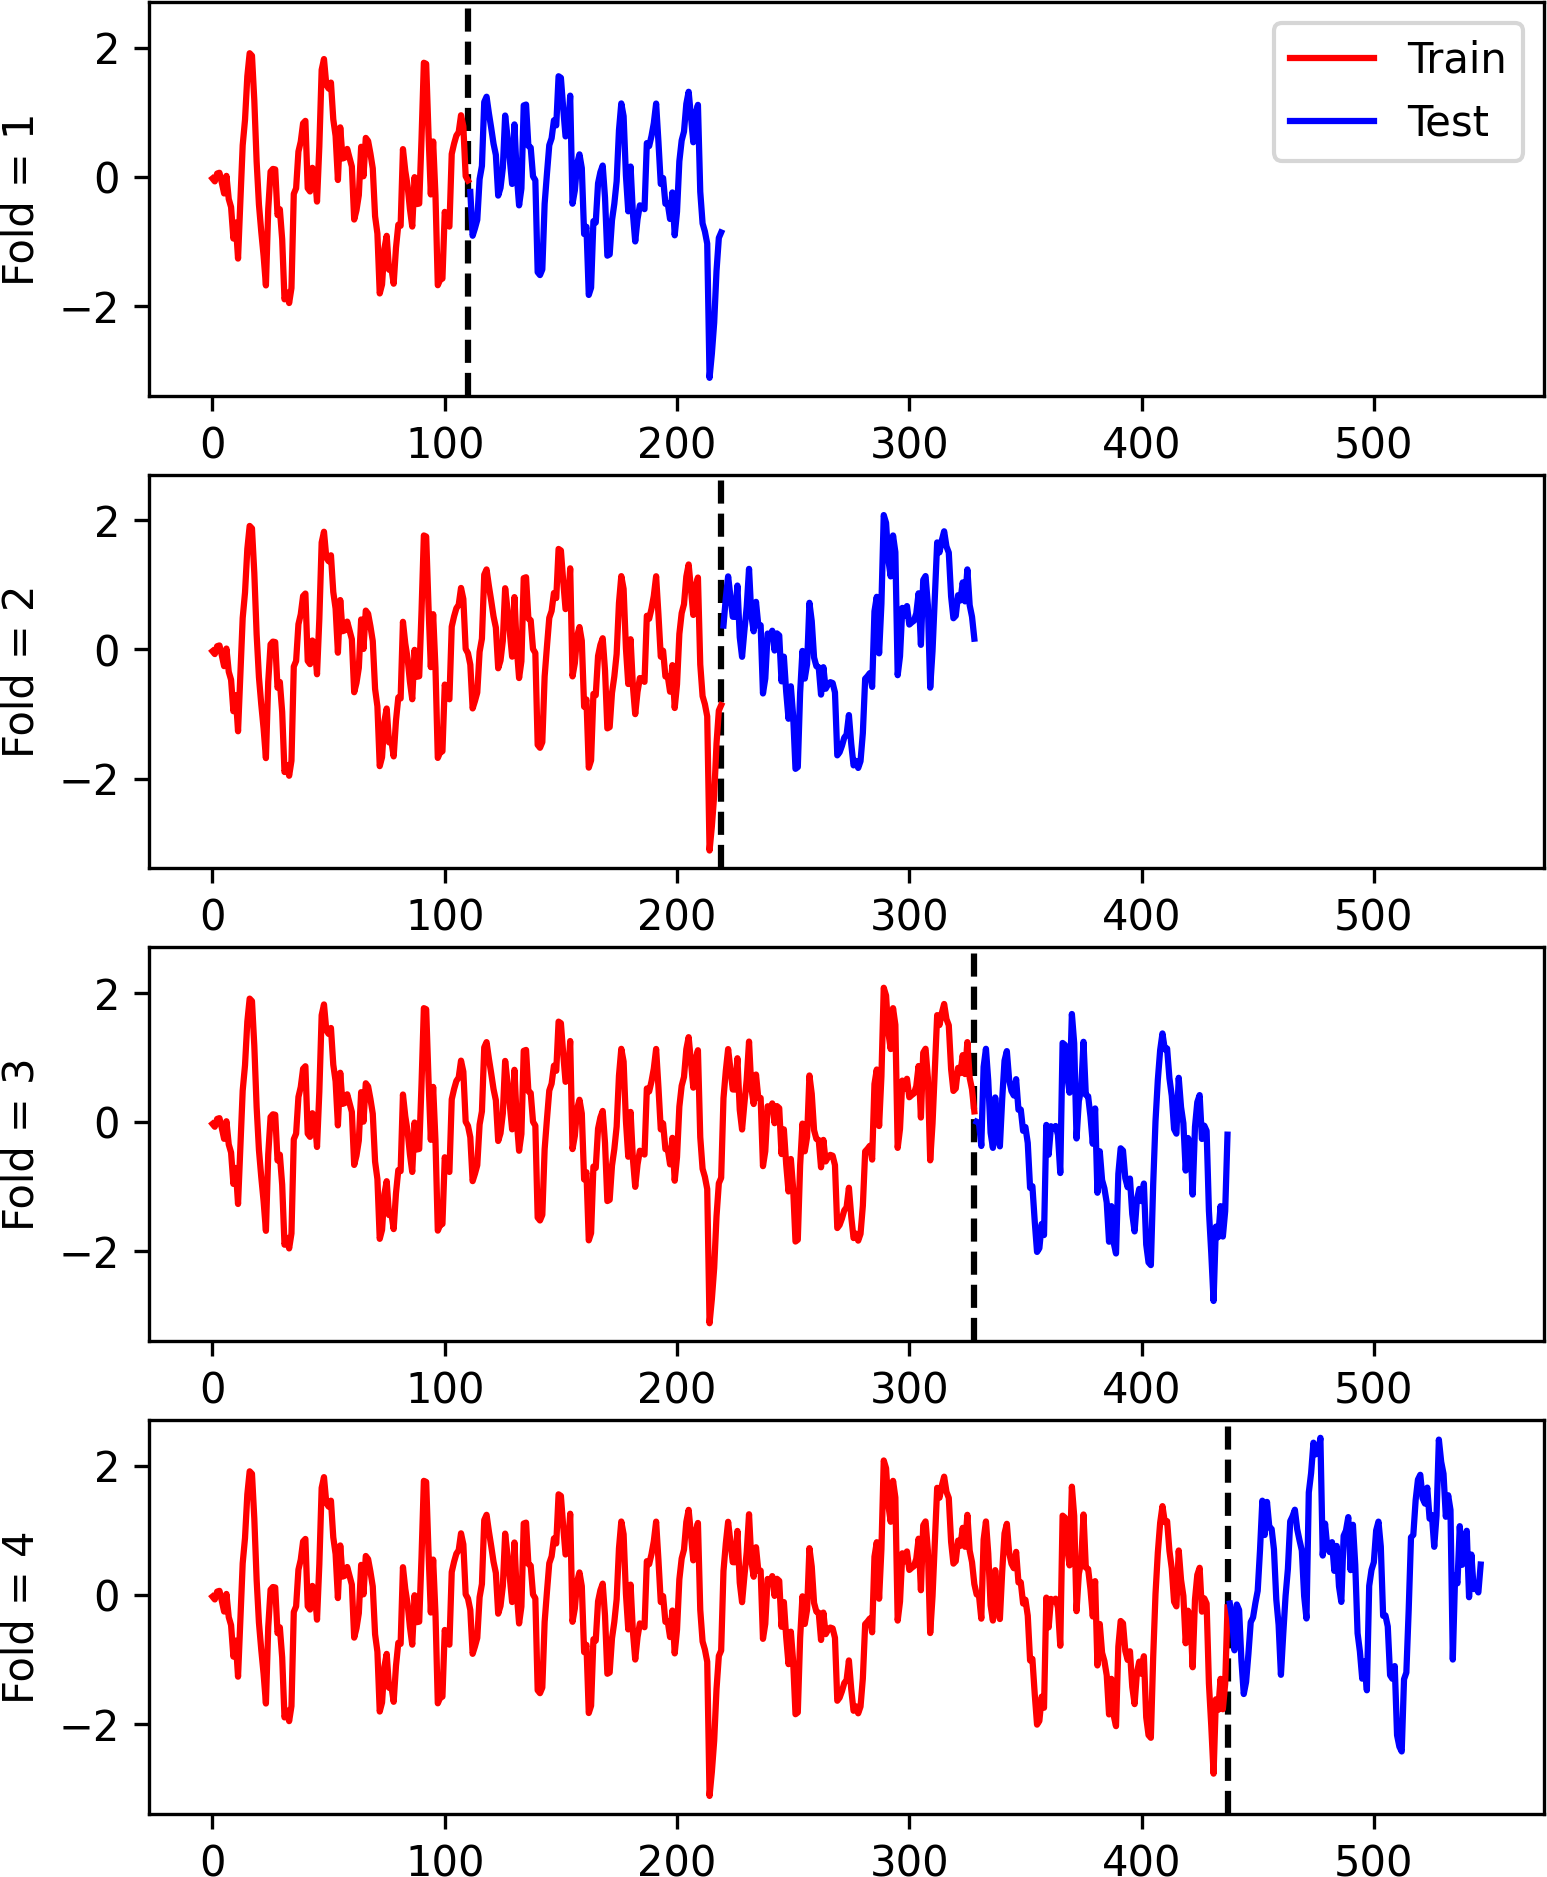
\includegraphics[width=0.6\linewidth]{./tscv.png}
\caption{\label{fig:tscv} Time series cross validation.}
\end{figure}


\subsection{Differential evolution}

Differential Evolution (DE) is a stochastic optimization algorithm, based on a population of solutions, which operates through computational steps similar to those employed by most Evolutionary Algorithms.
DE is simple and easy to implement, and it has some features such as superior performance in relation to accuracy, convergence speed and robustness, and few control parameters. %(F, Cr and NP).


The objective function, to be minimized by the differential evolution, is written as follows:
\begin{equation}
 f(x) = \mbox{RMSE}(x) * \left( 1 +  \frac{\beta}{N_{feat}} \sum_{i=1}^{N_{feat}} x_i^{MB}\right) 
\end{equation}
The parameter $\beta$ indirectly controls the complexity of the expressions generated for the linear model. From this equation, we observe when $\beta=0$ the resulting expression from the candidate solution is not penalized by its length.
As $\beta$ increases, expressions with a greater number of terms are more penalized than expressions with few terms. A proper choice of $\beta$ is crucial to balance the accuracy of the expression and the interpretability of the associated prediction model.


\section{Computational Experiments}\label{sec:results}


\section{Conclusion}\label{sec:conclusion}


% \section*{Compliance with Ethical Standards}
% 
% \subsection*{Funding}
% 
% \subsection*{Conflict of Interest/Competing Interest}
% The authors declare that they have no conflicts/competing interests.
%
% 
% \subsection*{Availability of data and material}
% Data and materials can be obtained upon request to the authors.
% 
% \subsection*{Code availability}
% Code can be obtained upon request to the authors.
% 


%
% ---- Bibliography ----
%
\bibliographystyle{spmpsci}
\bibliography{references}


\end{document}
